%%%%%%%%%%%%%%%%%%%%%%%%%%%%%%%%%%%%%%%%%%%%%%%%%%%%%%%%%%%%%%%%%%%%%%%%%%%%%%%%
%2345678901234567890123456789012345678901234567890123456789012345678901234567890
%        1         2         3         4         5         6         7         8

\documentclass[letterpaper, 10 pt, conference]{ieeeconf}  % Comment this line out
% if you need a4paper
%\documentclass[a4paper, 10pt, conference]{ieeeconf}      % Use this line for a4
% paper

\IEEEoverridecommandlockouts                              % This command is only
% needed if you want to
% use the \thanks command
\overrideIEEEmargins
% See the \addtolength command later in the file to balance the column lengths
% on the last page of the document

\usepackage[utf8]{inputenc}
\usepackage[T1]{fontenc}

% The following packages can be found on http:\\www.ctan.org
%\usepackage{graphics} % for pdf, bitmapped graphics files
%\usepackage{epsfig} % for postscript graphics files
%\usepackage{mathptmx} % assumes new font selection scheme installed
%\usepackage{mathptmx} % assumes new font selection scheme installed
\usepackage{amsmath}
%\usepackage{amssymb}  % assumes amsmath package installed
\usepackage{listings}
\usepackage{color}
\definecolor{dkgreen}{rgb}{0,0.6,0}
\definecolor{gray}{rgb}{0.5,0.5,0.5}
\definecolor{mauve}{rgb}{0.58,0,0.82}
\lstset{frame=tb,
    language=Python,
    aboveskip=3mm,
    belowskip=3mm,
    showstringspaces=false,
    columns=flexible,
    basicstyle={\small\ttfamily},
    numbers=none,
    numberstyle=\tiny\color{gray},
    keywordstyle=\color{blue},
    commentstyle=\color{dkgreen},
    stringstyle=\color{mauve},
    breaklines=true,
    breakatwhitespace=true,
    tabsize=3
}
\usepackage{graphicx}
\usepackage{hyperref}
\graphicspath{ {images} }

%%%%%%%%%%%%%%%%

\title{\LARGE \bf Title}

\author{Shun Ueda}

\begin{document}
    \maketitle
    \thispagestyle{empty}
    \pagestyle{empty}

    \subtitle{\textbf{GitHub Repo:} \url{https://github.com/shunueda/cse360-mobile-robotics/tree/lab-2}}


    \section{Part 1}

    \subsection{Exercise 5 - 2}

    Define the starting points ([1, 2] → [3, 3]).
    By using the equation provided, calculate the posistion and graph:

    \begin{lstlisting}[label={lst:lstlisting1}]
from numpy import array
from numpy.linalg import norm
from matplotlib.pyplot import figure, plot, show, xlabel, ylabel, title, legend, grid

K = 1
p_d = array([3, 3])
initial_position = array([1, 2], dtype=float)
time_step = 0.1
max_time = 10
tolerance = 0.1

positions = [initial_position.copy()]
current_position = initial_position.copy()
time_elapsed = 0

while norm(p_d - current_position) > tolerance and time_elapsed < max_time:
    u = K * (p_d - current_position)
    current_position += u * time_step
    positions.append(current_position.copy())
    time_elapsed += time_step

positions = array(positions)
    return np.array([ux, uy])
    \end{lstlisting}

    \begin{center}
        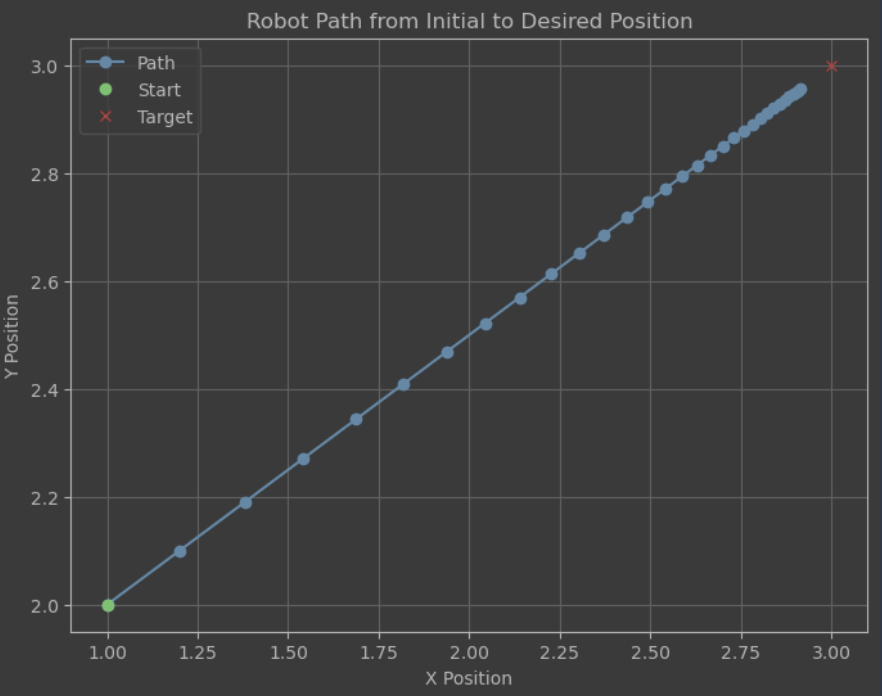
\includegraphics[scale=0.4]{1-1}
    \end{center}

    \subsection{Exercise 6 - 2}

    Define the waypoints, and calculate the position and graph (same as 5--2):

    \begin{lstlisting}[label={lst:lstlisting2}]
from matplotlib.pyplot import axis

waypoints = array([[-3, -3], [-2.8, 2.8], [3, -2.7], [2.9, 2.9], [0, 0]])

initial_position = waypoints[0]

positions = [initial_position.copy()]
current_position = initial_position.copy()
current_waypoint_index = 0
time_elapsed = 0

while current_waypoint_index < len(waypoints):
    p_d = waypoints[current_waypoint_index]
    if norm(p_d - current_position) < tolerance:
        current_waypoint_index += 1
        if current_waypoint_index == len(waypoints):
            break
        p_d = waypoints[current_waypoint_index]
    u = K * (p_d - current_position)
    current_position += u * time_step
    positions.append(current_position.copy())
    time_elapsed += time_step

positions = array(positions)
    \end{lstlisting}

    \begin{center}
        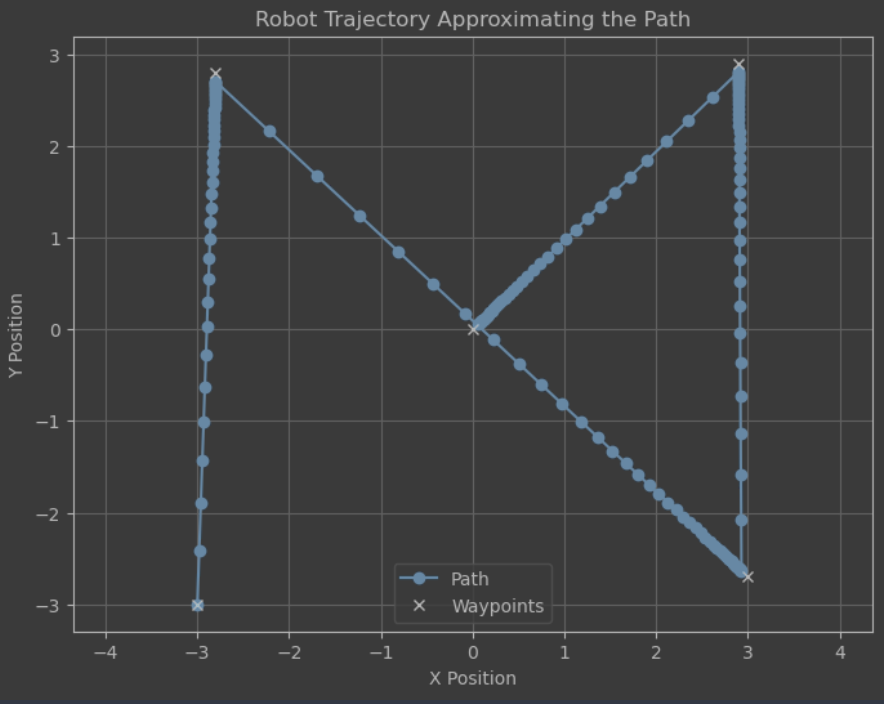
\includegraphics[scale=0.4]{1-2}
    \end{center}


    \section{Part 2}

    \subsection{Free Fall}

    Define the simulate function and calculate the position (using g = 9.8 in this case):

    \begin{lstlisting}[label={lst:lstlisting3}]
def simulate(dt, x, u, m=1, g=9.8):
    dx = array([x[3], x[4], x[5], 0, 0, -g])
    x += dt * dx
    if x[2] < 0:
        x[2] = 0
        x[5] = 0
    return x
    \end{lstlisting}

    The plotter is defined as follows.
    Since the motion is free fall, the force is only gravity, and the initial velocity is 0.

    \begin{lstlisting}[label={lst:lstlisting4}]
tf = 6
dt = 0.1
x = array([0., 0., 10., 0., 0., 0.])


def plotter(t):
    global x
    y = sense(x)
    u = control(t, y)
    x = simulate(dt, x, u)
    return x
    \end{lstlisting}

    \begin{center}
        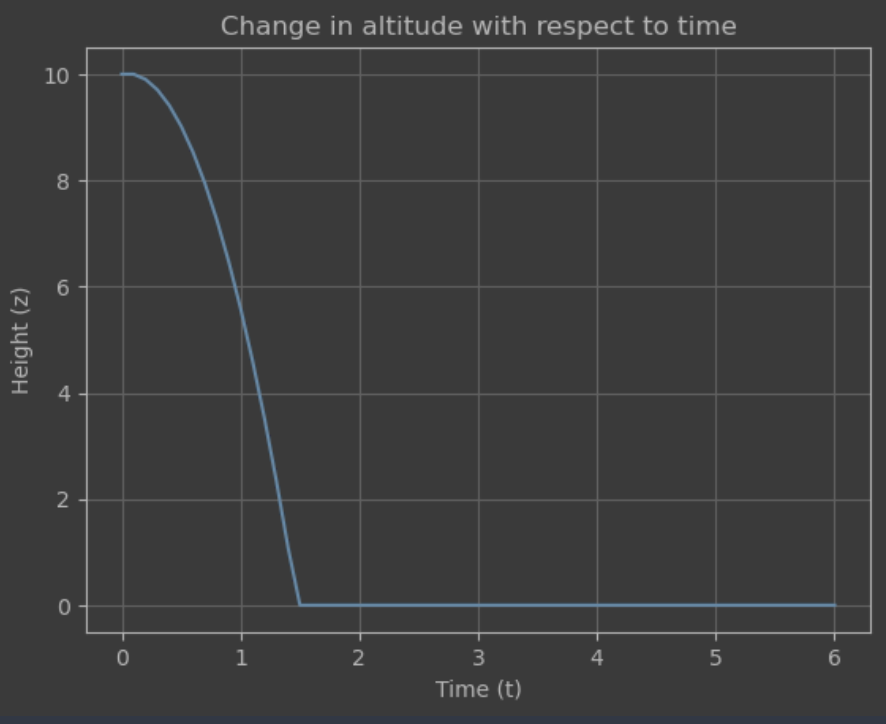
\includegraphics[scale=0.4]{2-1}
    \end{center}

    \subsection{Free Fall with Boyancy}

    Define the simulate function with buoyancy and calculate the position (using fb = 9.0 in this case):

    \begin{lstlisting}[label={lst:lstlisting5}]
def simulate_with_buoyancy(dt, x, u, m=1, g=9.8, fb=9.0):
    fg = m * g
    net_force = fg - fb
    net_acceleration = net_force / m
    dx = array([x[3], x[4], x[5], 0, 0, -net_acceleration])
    x += dt * dx
    if x[2] < 0:
        x[2] = 0
        x[5] = 0
    return x


tf = 6
dt = 0.1
x = array([0., 0., 10., 0., 0., 0.])
    \end{lstlisting}

    \begin{center}
        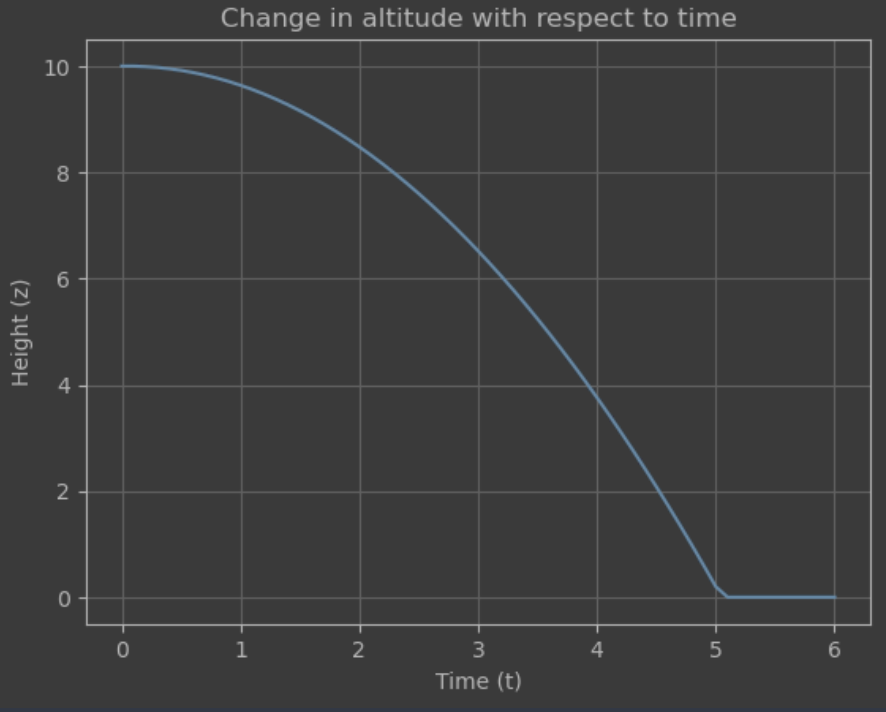
\includegraphics[scale=0.4]{2-2}
    \end{center}

    \subsection{Height Controller}

    Implement the height controller and calculate the position.
    Solve the IVP using the solve\_ivp function from scipy.integrate.

    \begin{lstlisting}[label={lst:lstlisting6}]
from numpy import linspace
from matplotlib.pyplot import figure, plot, xlabel, ylabel, title, legend, grid, show
from scipy.integrate import solve_ivp

g = 9.8
m = 1.0
z_d = 10
z_dot_d = 0
k_p = 100
k_d = 20


def dynamics(t, z):
    z_pos, z_dot = z
    u = k_p * (z_d - z_pos) + k_d * (z_dot_d - z_dot) + m * g
    z_ddot = (u / m) - g
    return [z_dot, z_ddot]


z0 = [0, 0]

t_span = [0, 1.5]
t_eval = linspace(t_span[0], t_span[1], 300)

sol = solve_ivp(dynamics, t_span, z0, t_eval=t_eval)
    \end{lstlisting}

    \begin{center}
        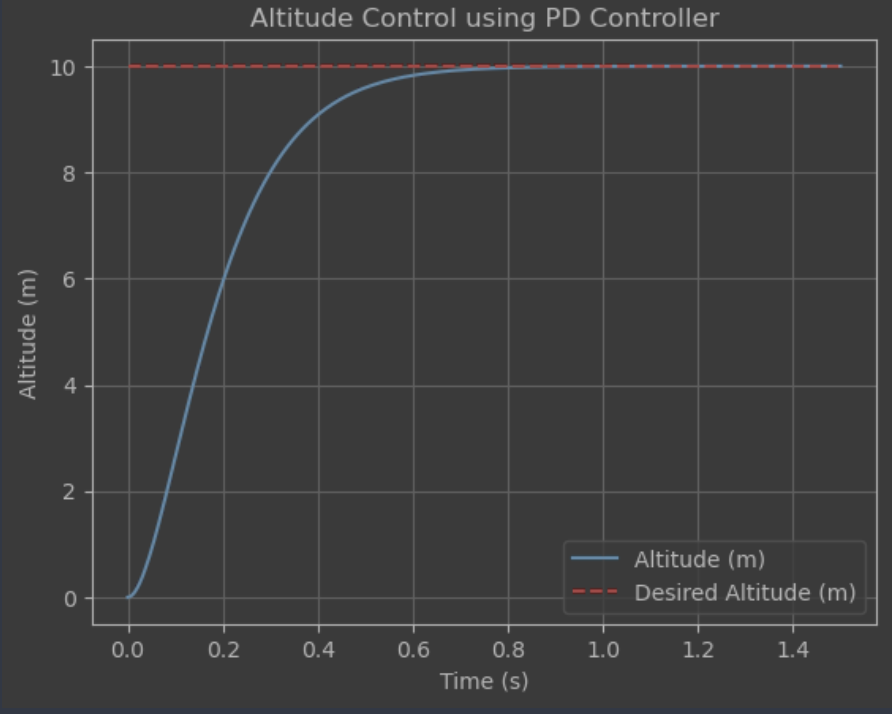
\includegraphics[scale=0.4]{2-3}
    \end{center}

    \subsection{Excercise 3 - 3}

    Implement the height controller with corrected mass and calculate the position.
    Consider the m\_actual and m\_estimated values, and solve the IVP using the solve\_ivp function from scipy.integrate.

    \begin{lstlisting}[label={lst:lstlisting7}]
from numpy import linspace
from matplotlib.pyplot import figure, plot, xlabel, ylabel, title, legend, grid, show
from scipy.integrate import solve_ivp

g = 9.8
m_actual = 0.8
m_estimated = 1.0
z_d = 15
z_dot_d = 0
k_p = 100
k_d = 20


def dynamics_corrected_mass(t, z):
    z_pos, z_dot = z

    u = k_p * (z_d - z_pos) + k_d * (z_dot_d - z_dot) + m_estimated * g

    u_corrected = u * (m_estimated / m_actual)
    z_ddot = (u_corrected / m_actual) - g
    return [z_dot, z_ddot]


z0 = [10, 0]

t_span = [0, 2]
t_eval = linspace(t_span[0], t_span[1], 300)

sol_corrected = solve_ivp(dynamics_corrected_mass, t_span, z0, t_eval=t_eval)
    \end{lstlisting}

    \begin{center}
        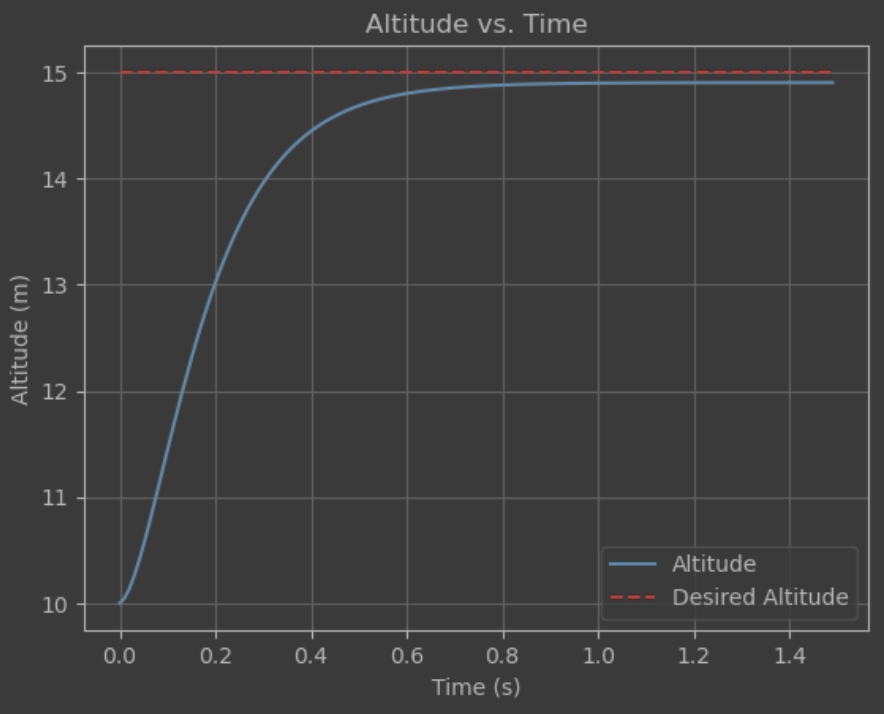
\includegraphics[scale=0.4]{2-4}
    \end{center}

\end{document}
